\chapter{Final Architecture}
\label{chap:final-architecture}

\section{Context Diagram}

\begin{figure}[H]
	\begin{centering}
		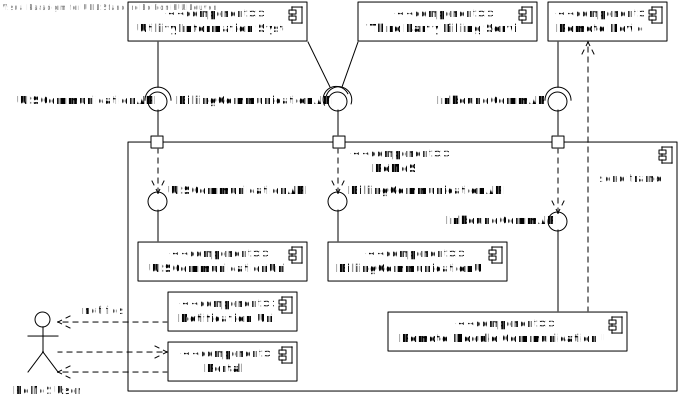
\includegraphics[width=\textwidth]{figs/final-context.pdf}
		\caption{The context diagram}
		\label{fig:final-context}
	\end{centering}
\end{figure}

\npar Figure \ref{fig:final-context} shows the context diagram. The ReMeS
user is a generalisation for all actors who can interact with the portal. 

\section{Overall Component Diagram}

\npar The overall component diagram is shown in figure
\ref{fig:final-components-left} and \ref{fig:final-components-right}.
Unfortunately, it is too large to fit one A4-sized paper. 

\begin{figure}[H]
	\begin{centering}
		\includegraphics[height=\textwidth,angle=-90]{figs/left-final-component.pdf}
		\caption{The component diagram of the overall system (left side)}
		\label{fig:final-components-left}
	\end{centering}
\end{figure}

\begin{figure}[H]
	\begin{centering}
		\includegraphics[height=\textwidth,angle=-90]{figs/right-final-component.pdf}
		\caption{The component diagram of the overall system (right side). The
		PredictionUnit is associated with the PredictionStorageAPI  and the BillingUnit is associated with
		the CustomerProfileAPI (on the previous page)}
		\label{fig:final-components-right}
	\end{centering}
\end{figure}

\section{Key Decompositions}

\npar In this section there will be a short overview of all iterations of the
ADD process, recapitulating every iteration by its corresponding interface
diagram. In every subsection there will be a link to the ADD chapter where to
find detailed information explaining all components and interfaces of the
diagram.

\subsection{Whole system}

\npar In diagram \ref{fig:final-architecture/it1} all the components of the
first iteration are shown. The explanation for the roles and responsibilities
respectively interfaces can be found in sections \ref{add:it1/elements} and
\ref{add:it1/interfaces}.

\begin{figure}[H]
	\begin{centering}
		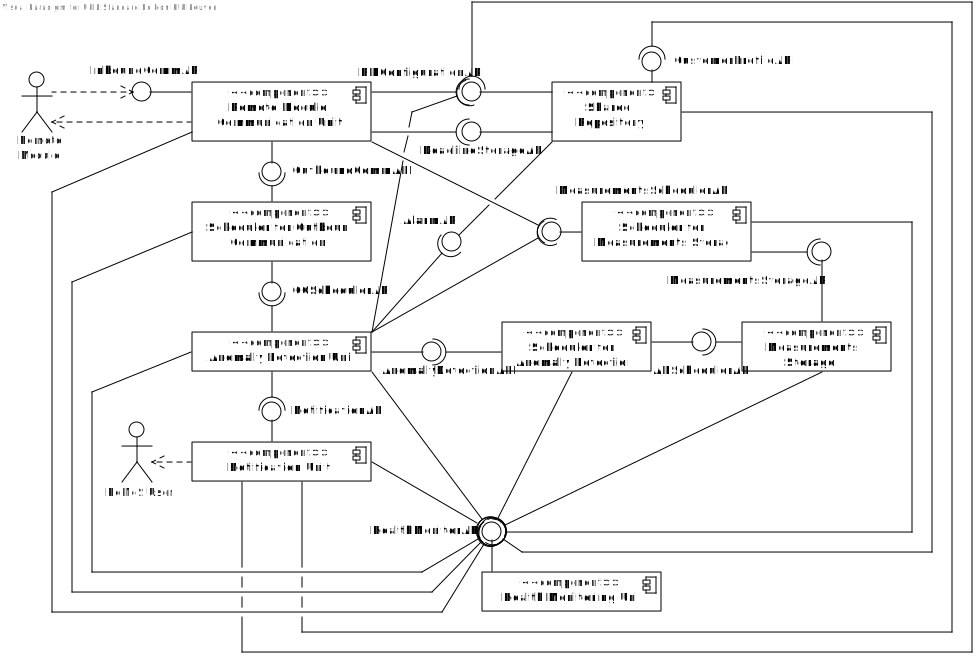
\includegraphics[width=1.4\textwidth,angle=90]{figs/add-it1-interfaces.pdf}
		\caption{Overview of the interfaces and components in the ReMeS
		System}
		\label{fig:final-architecture/it1}
	\end{centering}
\end{figure}

\subsection{Remote Module Communication Unit}

\npar The results of the second iteration are visualized in figure
\ref{fig:final-architecture/it2}. The corresponding components and interface
explanation can be found in respectively section \ref{add:it2/elements} and
\ref{add:it2/interfaces}.

\begin{figure}
	\begin{centering}
		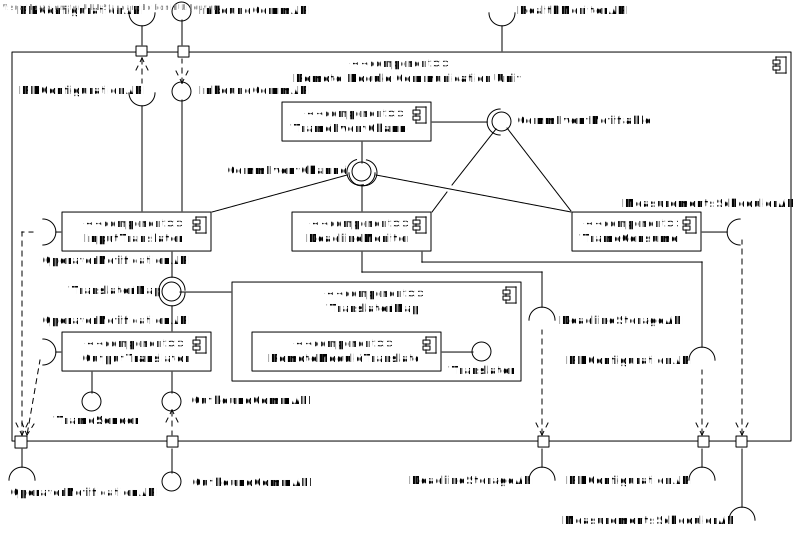
\includegraphics[width=\textwidth]{figs/add-it2-interfaces.pdf}
		\caption{Overview of the interfaces and components in the Remote
		Module Communication Unit.}
		\label{fig:final-architecture/it2}
	\end{centering}
\end{figure}

\subsection{Scheduler For MeasurementsStorage}

\npar Figure \ref{fig:final-architecture/it3} shows all the components of the
Scheduler for MeasurementsStorage, this was the third iteration. The roles and
responsibilties of each component can be found in \ref{add:it3/elements}. The
interfaces documentation is stated in section \ref{add:it3/interfaces}.

\begin{figure}
	\begin{centering}
		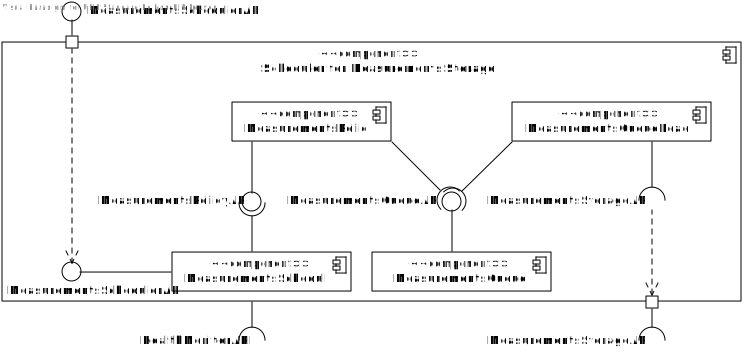
\includegraphics[width=\textwidth]{figs/add-it3-interfaces.pdf}
		\caption{Overview of the interfaces and components in the Scheduler For
		MeasurementsStorage.}
		\label{fig:final-architecture/it3}
	\end{centering}
\end{figure}

\subsection{MeasurementsStorage}

\npar The results of the fourth iteration are visible in figure
\ref{fig:final-architecture/it4}. Interface documentation can be found in
section \ref{add:it4/interfaces}. The component explanation is documented in
section \ref{add:it4/elements}.

\begin{figure}
	\begin{centering}
		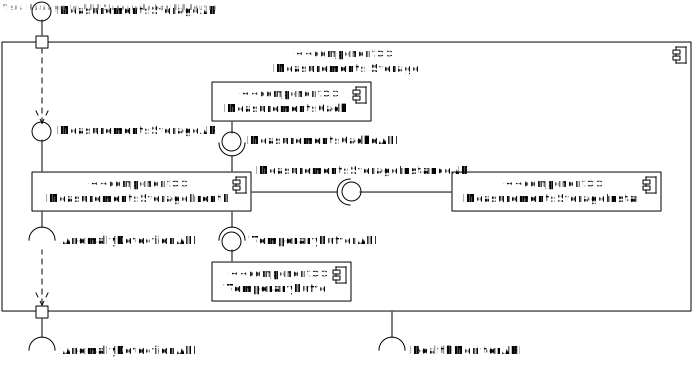
\includegraphics[width=\textwidth]{figs/add-it4-interfaces.pdf}
		\caption{Overview of the interfaces and components in the
		MeasurementsStorage.}
		\label{fig:final-architecture/it4}
	\end{centering}
\end{figure}

\subsection{Scheduler For Anomaly Detection}

\npar Iteration 5 discussed the decomposition of the scheduler for anomaly
detection. The results are shown in figure \ref{fig:final-architecture/it5}. The
component and interface documentation can be found in respectively section
\ref{add:it5/elements} and \ref{add:it5/interfaces}.

\begin{figure}
	\begin{centering}
		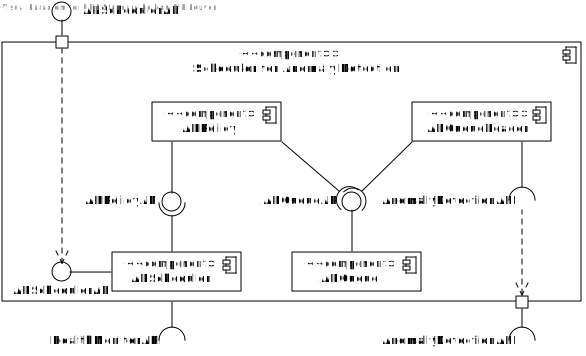
\includegraphics[width=0.9\textwidth]{figs/add-it5-interfaces.pdf}
		\caption{Overview of the interfaces and components in the Scheduler For
		Anomaly Detection.}
		\label{fig:final-architecture/it5}
	\end{centering}
\end{figure}

\subsection{Anomaly Detection Unit}

\npar In figure \ref{fig:final-architecture/it6} is the decomposition of the
Anomaly Detection Unit depicted. The explanation for the roles and
responsibilities of each component can be found in section
\ref{add:it6/elements}. The interface documentation is stated in section
\ref{add:it6/interfaces}.

\begin{figure}
	\begin{centering}
		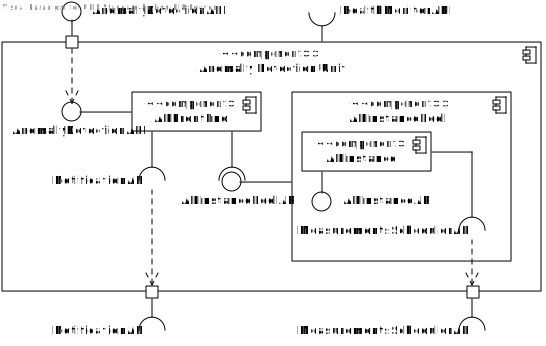
\includegraphics[width=\textwidth]{figs/add-it6-interfaces.pdf}
		\caption{Overview of the interfaces and components in the Anomaly Detection
		Unit.}
		\label{fig:final-architecture/it6}
	\end{centering}
\end{figure}

\subsection{Scheduler For Outbound Communication}

\npar The results of the seventh iteration are visualized in figure
\ref{fig:final-architecture/it7}. The corresponding components and interface
explanation can be found in respectively section \ref{add:it7/elements} and
\ref{add:it7/interfaces}.

\begin{figure}
	\begin{centering}
		\includegraphics[width=\textwidth]{figs/add-it7-interfaces.pdf}
		\caption{Overview of the interfaces and components in the Scheduler For
		Outbound Communication.}
		\label{fig:final-architecture/it7}
	\end{centering}
\end{figure}

\subsection{Notification Unit}

\npar Figure \ref{fig:final-architecture/it8} depicts the decomposition of the
Notification Unit. A detailed explanation of each component can be found in
\ref{add:it8/elements}. The interface documentation is to be found in section
\ref{add:it8/interfaces}.

\begin{figure}
	\begin{centering}
		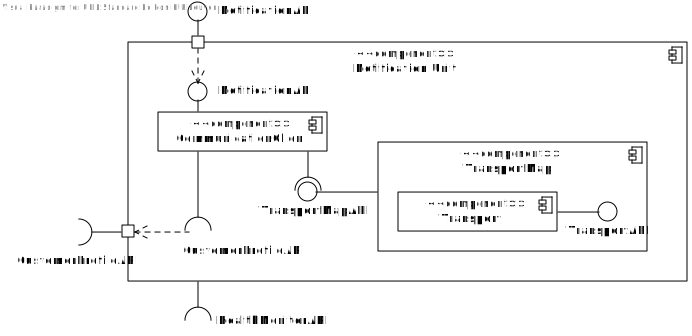
\includegraphics[width=\textwidth]{figs/add-it8-interfaces.pdf}
		\caption{Overview of the interfaces and components in the Notification Unit.}
		\label{fig:final-architecture/it8}
	\end{centering}
\end{figure}

\subsection{Health Monitoring Unit}

\npar Iteration 5 discussed the decomposition of the Health Monitoring Unit. The
results are shown in figure \ref{fig:final-architecture/it9}. The component and
interface documentation can be found in respectively section
\ref{add:it9/elements} and \ref{add:it9/interfaces}.

\begin{figure}
	\begin{centering}
		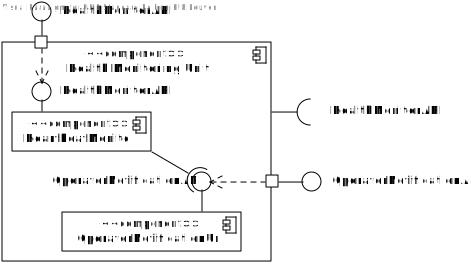
\includegraphics[width=0.7\textwidth]{figs/add-it9-interfaces.pdf}
		\caption{Overview of the interfaces and components in the Health Monitoring
		Unit.}
		\label{fig:final-architecture/it9}
	\end{centering}
\end{figure}

\subsection{Other}

\npar The final iteration, the tenth, contains the decomposition of the other
component. It is very important to remark that there never will be any notion of
an ``other component'' in the system once one starts implementing it. This can
also be seen in the overall component diagram, see
\ref{fig:final-components-left} and \ref{fig:final-components-right}.
Nonetheless is it shown in diagram \ref{fig:final-architecture/it10}, but it has
no functional meaning except for grouping the components. Documentation of the
components can be found in section \ref{add:it10/elements}. The interface
explanation is to be found in section \ref{add:it10/interfaces}.

\begin{figure}
	\begin{centering}
		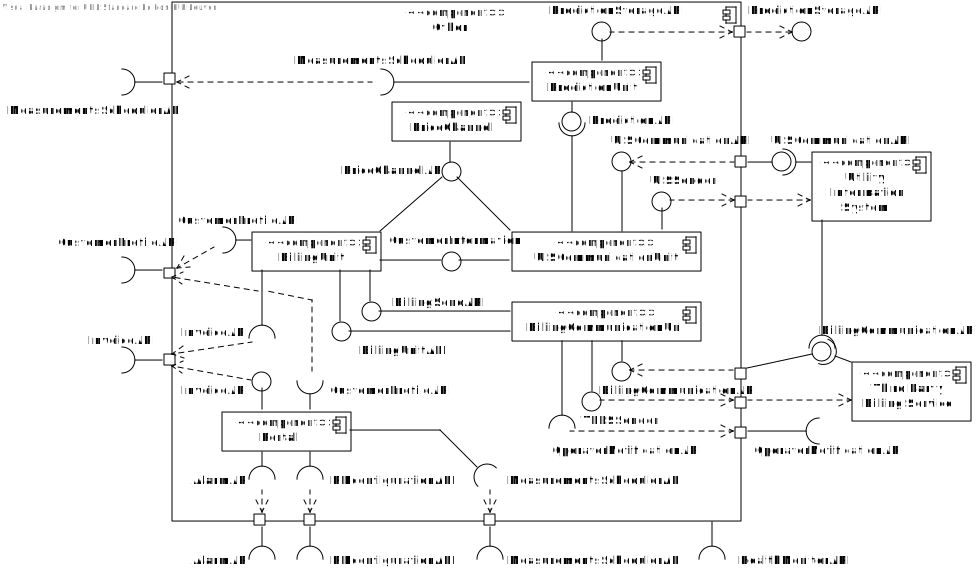
\includegraphics[width=1.4\textwidth,angle=90]{figs/add-it10-interfaces.pdf}
		\caption{Overview of the interfaces and components in the Other component.}
		\label{fig:final-architecture/it10}
	\end{centering}
\end{figure}

\section{Deployment Diagram}

\npar The deployment diagram is shown in figure \ref{fig:final-deployment}. 

\begin{figure}
	\begin{centering}
		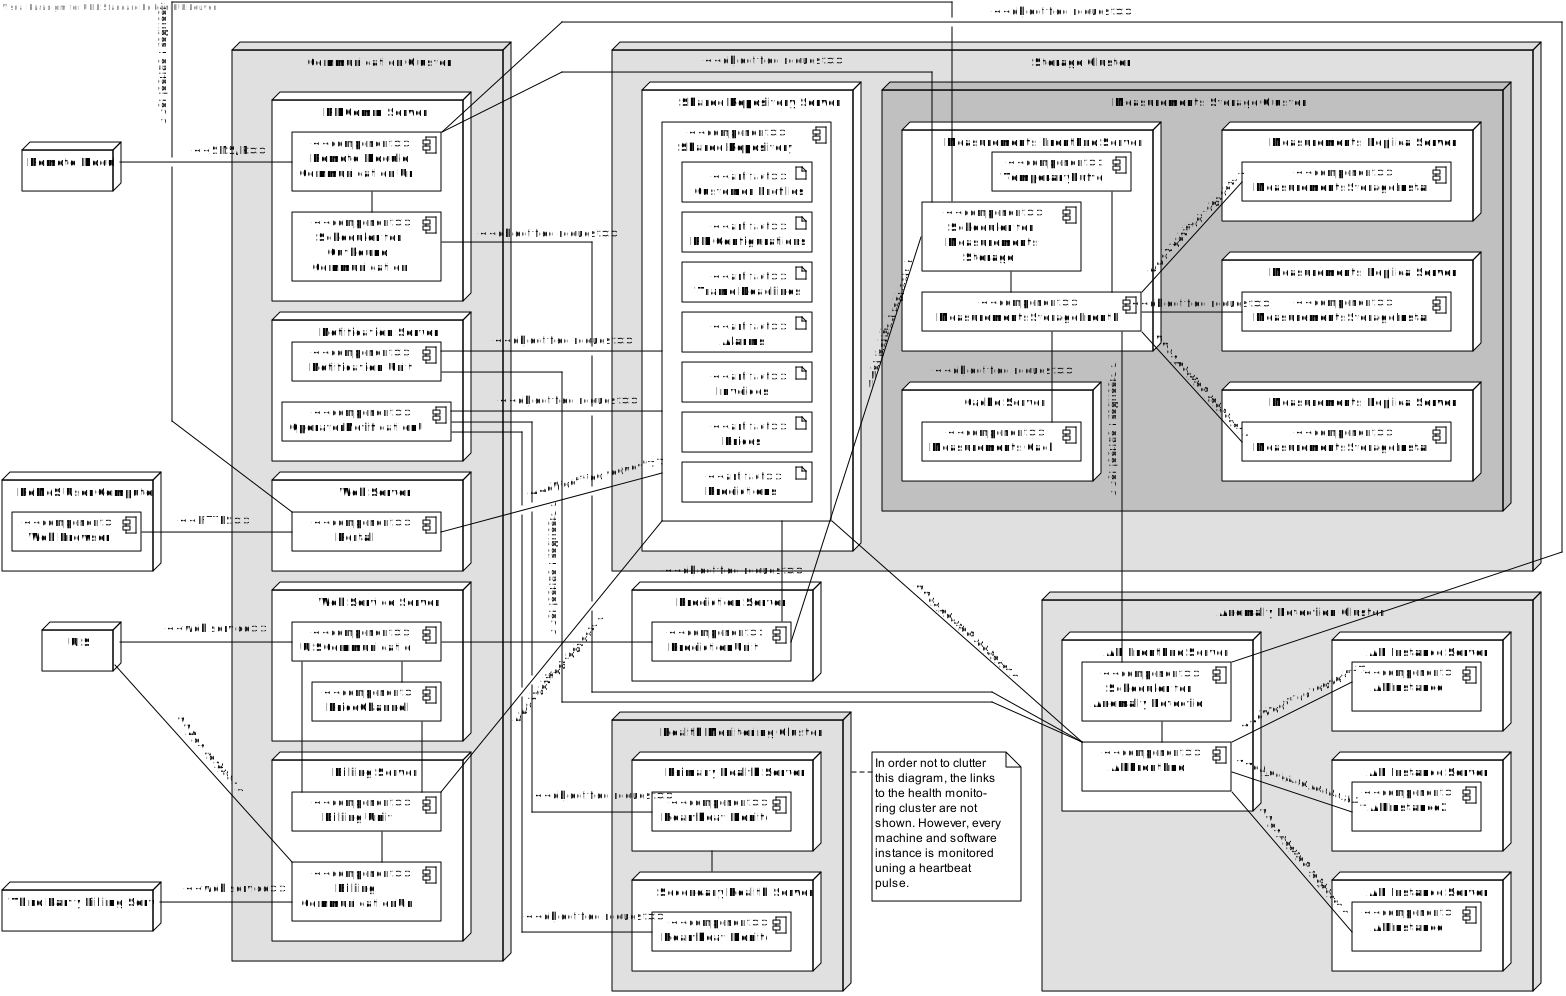
\includegraphics[width=1.42\textwidth,angle=90]{figs/final-deployment.pdf}
		\caption{The deployment diagram}
		\label{fig:final-deployment}
	\end{centering}
\end{figure}

\npar A trame always arrives at the RMComm Server in the Communication Cluster.
This server acts as a gateway for all remote module communication. It will also
host the scheduler for outbound communication. To summarize, the RMComm Server
is responsible for all trame communication. 

\npar As already mentioned, the Communication Unit will route trames to the
right units: a measurement trame is routed to storage, an alarm trame is
immediately routed to the anomaly detection unit. Both units have been assigned
their own clusters: the measurements storage cluster and the anomaly detection
cluster.

\npar The anomaly detection cluster exists of a frontend server, which takes
care of scheduling, resource arbitration and results processing
(shutting the valve and dispatching the notification unit in case of an alarm).
Among the frontend server, there are a number of anomaly detection instances.
Only three are shown but additional instances can be easily added and/or
removed. This is one of the advantages of the resource pool design pattern.

\npar The measurements storage cluster is contained in a general storage
cluster. Again, as with the anomaly detection cluster, the scheduler, frontend
and buffer are assigned to a single machine. That machine communicates with a
cache server and multiple measurements storage replicas. 

\npar Among the measurements storage cluster, there is a shared repository
server. This machine handles all other storage, from customer profiles to
predictions and historical prices. 

\npar Every machine in the deployment diagram communicates with the heartbeat
cluster. This is, however, not shown in figure \ref{fig:final-deployment}
because it would only make the diagram less clear. This cluster has a primary
server and a secondary server, which monitors the primary and vice versa. This
way, virtually 100\% of both servers can be guaranteed. What is the chance that
both servers fail at exactly the same time?

\npar The notification of ReMeS operators is handled by the Notification Server.
This server is also used to notify alarm recipients and the customer in case of
an alarm. 

\npar The billing is separated from the rest of the system because it is an
expensive operation, happens only once a month and should not affect the
operation of the other systems. 

\npar A similar reasoning is used for the Prediction Server. This is an
expensive operation that should not interfere with the other systems and runs
less often than the other systems.

\npar Communication with the UIS is provided through the Web Service Server. It
is assumed that communication with third parties will be implemented with web
services. 

\npar Last, but not least, a webserver provides access to all ReMeS data. The
traffic between the user's browser and the web server is encypted.

\npar The deployment diagram is created with the idea that is is probably better
to define multiple small, easy replacable machines instead of few, large
do-it-all servers. With the current virtualization technologies, the hardware of
multiple nodes in this system can be shared, which will reduce hardware and
maintenance costs.